\documentclass{article} % For LaTeX2e
\usepackage{nips12submit_e,times}
\usepackage{amsmath,amsthm,amssymb, dsfont}
\usepackage{pgf, tikz}
\def\I{\mathbb{I}}
\usetikzlibrary{arrows,automata}

\title{Infectious Knowledge in Collaborative Social Sites}


\author{
Eliana Feasley\\
Department of Computer Science\\
University of Texas at Austin\\
\texttt{elie@cs.utexas.edu} \\
\And
Wesley Tansey\\
Department of Computer Science\\
University of Texas at Austin\\
\texttt{tansey@cs.utexas.edu} \\
}

\newcommand{\fix}{\marginpar{FIX}}
\newcommand{\new}{\marginpar{NEW}}
\def\c{\textbf{ Cite }}
\nipsfinalcopy

\begin{document}

\maketitle

\begin{abstract}
In recent years, the attention paid to cascading information in social networks has been increasing in a fashion itself comparable to a social cascade. This makes sense - the way that information infects different spaces of ideas has applications to basic graph theory, epidemiology, predictions of the future, and marketing. In this paper, we examine the dynamics of information spread across subcommunities with overlapping networks in several domains - the question-answering site \texttt{StackExchange}, a news network provided by memetracker, and a synthetic dataset of our own devising. Each of these is structured such that it is possible to track how ideas spread over time, and to discover semi-explicit communities and the connections between them.
\end{abstract}

\section{Introduction}
\label{intro}
Social cascades capture the concept of new ideas, or \textit{memes}, spreading across influence networks and infecting subcultures. Cascade theory has applications to several areas, including epidemiology, graph theory, machine learning, and marketing. In this paper, we examine the dynamics of information-spread across sub-communities with overlapping networks in several real-world domains: the social news site \textit{reddit}, a collection of blogs and mainstream media \cite{memetracker}, and the question-answer network \textit{StackExchange}. Our goal is to capture the flow of memes by learning a graphical model for each domain. We present approaches for inferring both the structure and weights of such models.

Information online travels across networks in a variety of configurations, and it is easy to see information spreading across them. 
Our work is an extension of the NetInf work \cite{netinf}, in which the authors learn the structure of a graph from observing cascades. Where as the NetInf 

In this paper, we explore how modeling this mechanism as a timeseries can help us both to predict future topics and to discover the structure of latent communities.

The remainder of this paper is organized as follows. Section \ref{sec:background} presents an overview of previous work on cascades. Section \ref{sec:structure} presents our algorithm for approximate structure learning in collaborative sites. Section \ref{sec:prediction} details the results of using graphical models to predict social cascades. Finally, section \ref{sec:conclusions} discusses potential future work and concludes.

\section{Background}
\label{sec:background}
The rise of online social media in recent years has created numerous opportunities for social cascade researchers. In this section, we discuss some of the work performed on cascades in social media, compare their applicability to collaborative sites, and differentiate them from our own approach.

\subsection{Collaborative Sites}
A \textit{collaborative site}, in this paper, is defined as any site which has a single overall userbase and multiple subsites. Each user in the site is subscribed to at least one subsite and can optionally choose to subscribe to as many of the subsites as they like. Examples of such sites may include social news sites, question-answer sites, and discussion forums. Note that traditional friendship social networks are not valid collaborative sites, as users must be given permission to \textit{friend} other users. Similarly, microblogging sites do not qualify, as users are not able to comment directly on another user's feed.

\subsection{Social Cascades}
In \cite{info_contag} the authors use the explicit struture of networks - observing following and friendship relationships in order to explore the effect of actual, instead of inferred, network structure on information cascades. They observe that the popularity of stories peaks with an age of about one day, and then subsides. 

A unique aspect of open networks like reddit\footnote{http://reddit.com} and digg\footnote{http://digg.com} is that it is possible for information to latently travel quickly, as opposed to in closed, action oriented networks like the one described in \cite{viral_dynamics}, where information, which must individually be spread from one email to another, peters out quickly.

In \cite{twitter_trend}, the authors identify \textit{``bursty''} keywords that suddently appear, and attempt to align them with trends \dash entire topics that are becoming more popular. In collaborative sites, however, we are interested in both the rise of such topics and the path they travel through the network of subsites.

\subsection{Structure Learning}
Inferring networks of influence has been studied in a variety of contexts. Contagion networks have been used \cite{contagion} to model the spread of disease throughout a social network. 
As internet domains are fully connected, and inference over fully connected graphs is intractable, it is important to 
% OUR STORY; Learning social networks is important. Past att
\section{Learning Structure}
\label{sec:structure}
In this section, we present our approach to learning the structure of influence graphs in collaborative sites. We first present an overview of the general problem, followed by our approach to learning structure, and finally validate our approach by learning structure graphs for two real-world datasets, \textit{reddit} and \textit{StackExchange}.

\subsection{Challenges for Collaborative Sites}
Learning graphical model structure is a particularly difficult task for collaborative sites. Each subsite forms a node in the network, and memes can potentially between any two subsites that share at least one user in common. Typically in social networks, we expect the percentage of mutual friends to be relatively low and edges exist simply as binary friend-or-not connections. However, in collaborative sites with thousands of users, it is reasonable to expect that every subsite shares at least one user in common. A naive approach would thus result in a fully connected graph, which is undesirable as it reveals little insight and may make certain tasks intractable.

\subsection{Approximate Structure Learning Algorithm}
Since it is possible for a meme to spread between any two subsites, any structure learning algorithm that yields a less-than-fully-connected graph is learning an approximate structure. As noted previously, an approximate structure may be desirable for gaining insights and reducing computational requirements. We next present our approximate structure learning algorithm for collaborative sites.

We first begin by defining an \textit{adjency matrix}, $\mathcal{A}$, over subsites. For each pair, $(s,t) \in \mathcal{A}$, of subsites, we mine the percentage of \textit{active} users that overlap in both $s$ and $t$. We define a user as \textit{active} if they have posted at least once on both subsites\footnote{Note that mining inactive users would be infeasible since most collaborative sites have user subsite subscriptions as private.}:

$$
\mathcal{A}[s,t] = \sum_{\forall u \in \mathcal{U}}\dfrac{a(u)}{min(|\mathcal{U}^s|,|\mathcal{U}^t|)}$$
$$
a(u) = \begin{cases}1&u \in P_s\text{ and }u \in P_t\\0 &\text{otherwise}\end{cases}
$$

Where $\mathcal{U}$ is the set of users and $P_i$ is the set of posts in subsite $i$.

Rather than focusing on binary co-occurrence edges, our algorithm assesses the strengths of user overlap between two subsites and removes edges that are below a user-specified threshold. We define the relative strength matrix, $\mathcal{A}^*$:

$$
\begin{array}{lll}
\mathcal{A}^*[s,t] &=& \dfrac{\mathcal{A}[s,t] - \mu(\mathcal{A})}{\sigma(\mathcal{A})}\\
\end{array}
$$

Where $\mu$ and $\sigma$ are the mean and standard deviation, respectively. Finally, we define the weighted edge matrix, $\mathcal{E}$:

$$
\begin{array}{lll}
\mathcal{E}[s,t] &=& \begin{cases}\mathcal{A}^*[s,t] & \text{if }\mathcal{A}^*[s,t] \geq \gamma \\0 &\text{otherwise}\end{cases}\\
\end{array}
$$

Where $\gamma$ is the user-specified strength threshold.

The resulting graph, $\mathcal{G} = (\mathcal{S},\mathcal{E})$, captures the most likely sources of influence for each node. To predict meme spreads, one could then convert $\mathcal{G}$ to a dynamic graphical model, $\mathcal{G}^*$, that captures the transition from $\mathcal{G}$ to $\mathcal{G'}$:

$$
\begin{array}{lll}
\mathcal{G}^* &=& (\mathcal{S}^*,\mathcal{E}^*)\\
\mathcal{S}^* &=& S \cup S'\\
\mathcal{E}^*[s,t] = &=& \begin{cases}1 & \text{if } s \in \mathcal{S}\text{, }t \in \mathcal{S'} \text{, and } \mathcal{E}[s,t] > 0\\
                                      1 & \text{if } s \in \mathcal{S'}\text{, }t \in \mathcal{S'} \text{, and } \mathcal{E}[s,t] > 0\\
                                      0 & \text{otherwise}\end{cases}\\
\end{array}
$$

Queries to our dynamic graph will always be performed with the nodes in $\mathcal{G}$ being observed, thus connecting them would not affect the MAP inference for nodes in $\mathcal{G'}$. One important point is that while the weights inferred by our algorithm could represent final weights in a graphical model, it is not clear that doing so would produce high accuracy.

\subsection{Experiments}
To validate our approach, we mined active user adjacency matrices for three real-world collaborative sites: \textit{reddit}, \textit{StackExchange}, and \textit{SomethingAwful}. The results for each site are presented next.

\subsubsection{reddit}
\textit{reddit} is a social news site where each subsite\footnote{reddit subsites are called subreddits.} represents a different news topic. By default, all users are subscribed to a generic set of subsites such as \textit{politics} and \textit{humor}. The overlap among these default subsites is very high resulting in very little signal in the adjacency matrix; it is also worth noting that these subsites are more likely to be the final destination of memes, given that they are less niche than the non-default subsites. Consequently, we first removed all default subsites from our dataset. To conform to our time constraints and maximize the amount of insight we could draw, we then limited the remaining non-default subsites to only the top 25. The resulting graph generated by our structure learning algorithm is shown in Figure \ref{fig:reddit}.

Two interesting properties of the graph immediately stand out. First, the explicit-content subreddits, \textit{nsfw}, \textit{sex}, and \textit{gonewild}, are clustered together, indicating that memes on these subreddits are not likely to spread to the rest of the network and memes within the cluster will quickly infect the remaining nodes. Conversely, the marijuana-oriented subreddit, \textit{trees}, is a super-node that appears to exert influence on nearly every node and vice-versa. Intuitively, we may thus hypothesize that the users of \textit{trees} are very influential on reddit and would thus expect to see memes spread from and to \textit{trees} rapidly.

\begin{figure}[htb]
\centering
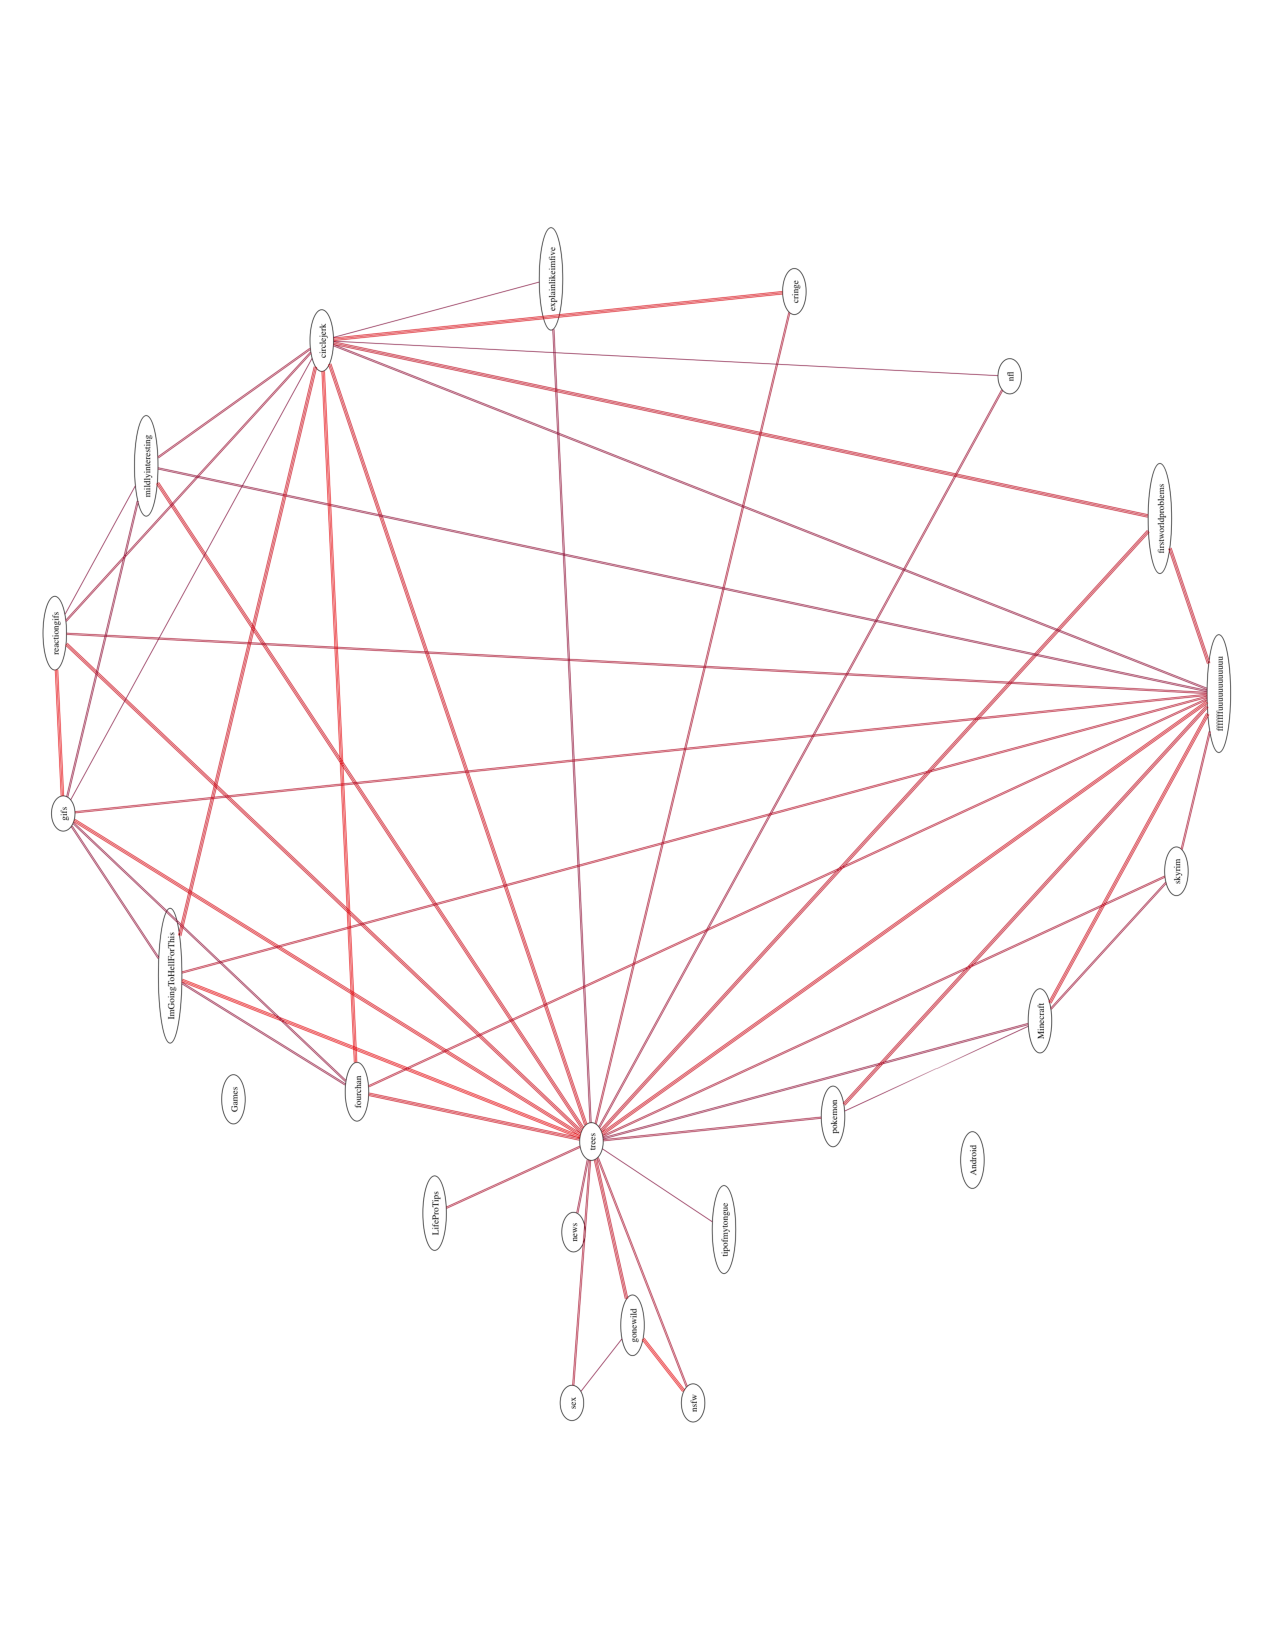
\includegraphics[width=\textwidth]{reddit.pdf}
\caption{Graph inferred from the top 25 non-default subreddits.}
\label{fig:reddit}
\end{figure}

\subsubsection{StackExchange}
\textit{StackExchange} (SE) is a collaborative question-answer site where each subsite represents a different question topic. A majority of subsites focus on technical topics such as \textit{android} and \textit{security}, though non-technical subsites exist (e.g., \textit{cooking}). Memes in SE are more likely to take the form of rising topics of interest, such as the popularity of iPhone games or Ruby on Rails, rather than cultural topics like on reddit. Unlike most collaborative sites, SE user subscription data is publicly available. We therefore used the adjacency matrix of all users to build our graph. The resulting graph for SE is shown in Figure \ref{fig:stackexchange}.

Perhaps counter-intuitively, the \textit{stackoverflow} subsite has two orders of magnitude more overall users than other sites, but exerts no influence on the network. This may be a result of the other subsites being relatively unknown but having a strong sub-culture of shared users. Two high-influence pseudo-clusters appear between less technical and strictly technical sites in the upper-left and lower-right, respectively. Thus, we would expect that localized memes would be frequent among these pseudo-clusters.

\begin{figure}[htb]
\centering
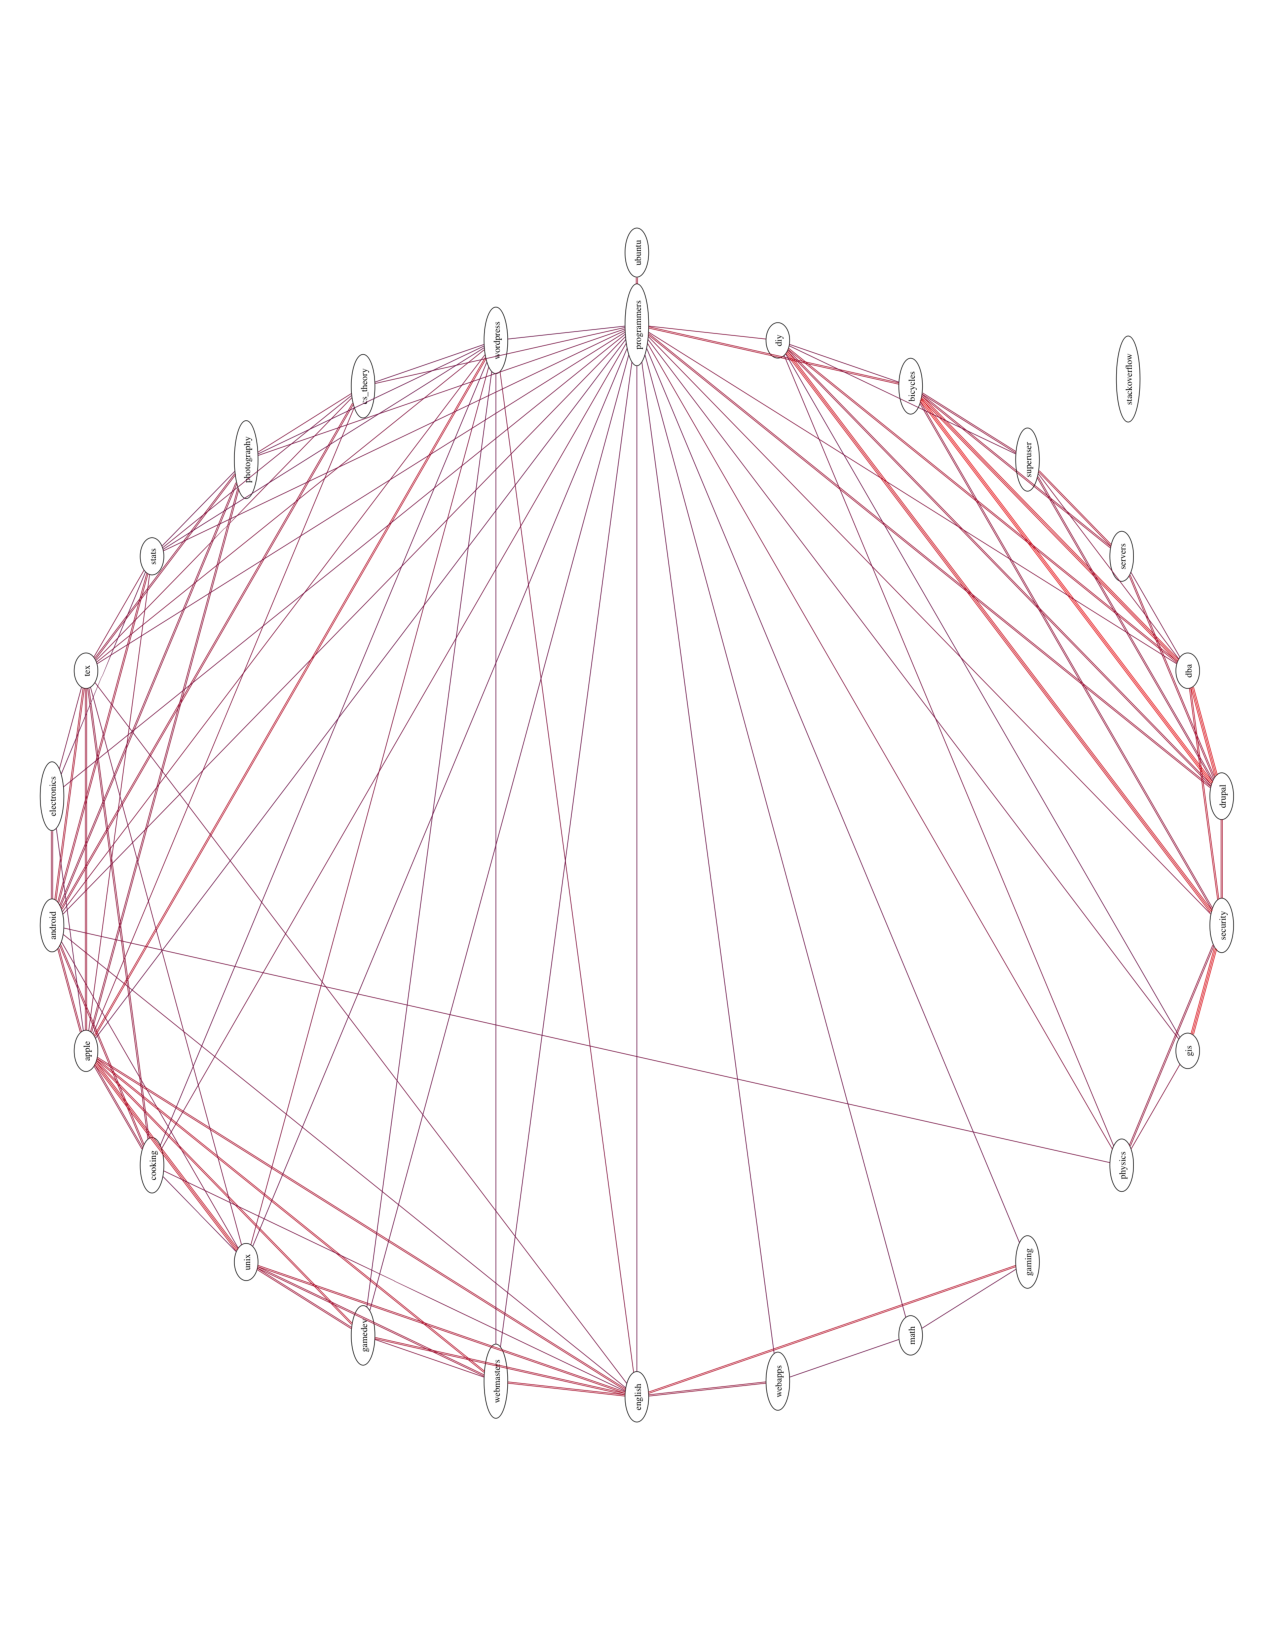
\includegraphics[width=\textwidth]{stackexchange.pdf}
\caption{Graph inferred from the 28 StackExchange subsites.}
\label{fig:stackexchange}
\end{figure}

\subsubsection{SomethingAwful}


\section{Predicting Cascades}
\label{sec:prediction}

The second task is a difficult inference problem, detecting cascades in networks of sites. This task has two components - learning the connections between the sites and using the strengths of these connections to predict the sites of future infections. In \cite{netinf}, the authors learn the strength of connections between sites to visualize and explore the data, while we extend this research by using connections to predict future data.


\subsection{Problem statement}
Given nodes $\mathcal{D}$ with overlapping connections $\mathcal{C}$ via shared users, predict topic vector $v_{d,t+1}$ in document collection $d$ at time $t+1$ given the topics $V$ in all documents at time $t$?


Following the model in \cite{influential}, we refer to a node as \textit{contagious} for a given phrase if it has had that phrase trend internally within the last timestep. A node that contains a previously trending phrase can be viewed as having become \textit{infected.} 

Given sites $\mathcal{D}$ with overlapping connections $\mathcal{C}$ via shared users, predict topic vector $v_{d,t+1}$ in site $d$ at time $t+1$ given the topics $V$ in all documents at time $t$.

Following the model in \cite{influential}, we refer to a node as \textit{contagious} for a given phrase if it has had that phrase trend internally within the last timestep. A node that contains a previously trending phrase can be viewed as having become \textit{infected.} 

We model this domain as an unfolding Markov Chain, in which at each timestep, nodes become infected or uninfected. See the below graph, in which nodes $\{A,B,C\}$ represent the states of three sites at time $t$, and the nodes $\{A',B',C'\}$ represent the same nodes at time $t+1$.

\subsection{Problem Structure}

As infections spread over continuous time but our model involves only discrete timesteps, our model must account for the fact that newly infected nodes may cross-contaminate. Towards this end, we connect all of the nodes in the second timestep.

The number of nodes in both timesteps $|V|=2|S|$, with $S$ being the set of all sites. The number of edges $|E|=\frac{3}{2}|S|^2 - S$ - $S^2$ captures influence between each site at time $t$ and each site at time $t+1$, and between each site at time $t+1$ with every other such site.

$$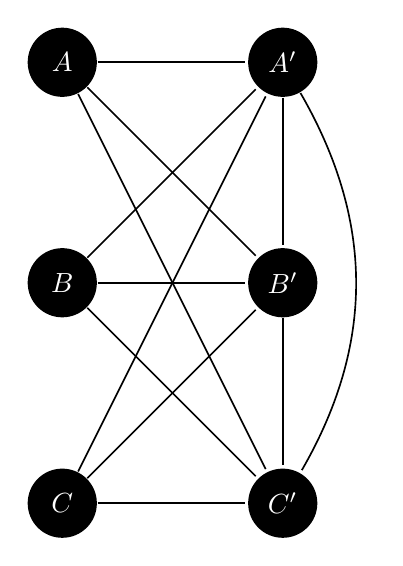
\begin{tikzpicture}[-,>=stealth',shorten >=1pt,auto,node distance=2.8cm,
                    semithick]
  \tikzstyle{every state}=[fill=black,draw=none,text=white]

  \node[state] (A)                    {$A$};
  \node[state]         (B) [below of=A] {$B$};
  \node[state]         (C) [below of=B] {$C$};
  \node[state]         (A1) [right  of=A] {$A'$};
  \node[state]         (B1) [right of=B] {$B'$};
  \node[state]         (C1) [right of=C] {$C'$};


  \path (A) edge        node {} (A1)
        (A) edge        node {} (B1)
        (A) edge        node {} (C1)
        (B) edge        node {} (A1)
        (B) edge        node {} (B1)
        (B) edge        node {} (C1)
        (C) edge        node {} (A1)
        (C) edge        node {} (B1)
        (C) edge        node {} (C1)
        (A1) edge        node {} (B1)
        (A1) edge [bend left] node {} (C1)
        (B1) edge        node {} (C1);
\end{tikzpicture}
$$

The number of nodes $|V|=2|S|$, with $S$ being the set of all sites. The number of edges $|E|=\frac{3}{2}|S|^2$

\subsection{Detecting Infections}
\label{infections}

To detect infections, we use Pointwise Mutual Information \cite{pmi} to identify salient bigrams in each site in each timestep. Whenever these occur multiple times across the entire dataset, they may be infections. We examine the occurences of each ngram to see if it appears in bursts, and if it does, we designate it an infection.


\subsection{Learning Parameters}


We used the method for finding the MLE estimate in triangulated graphs described in \cite{wainwright} to learn the weights of our edges. The model is trained on every pairs of steps $t,t+1$. We define indicator functions 
$$\I[s]=\begin{cases}1&$Infection occurs in site $s\\0& s $ is not uninfected$\end{cases}$$ 
and
$$\I[s,t;j,k]=\begin{cases}1&$if infection is present in site $s$ ($j=1$) and $t$ ($k=1$)$\\
0& $otherwise$\end{cases}$$ 

Parameters are the logs of the expectations of these indicator functions.


\subsection{Inference Problem}
Our question “Given a cascade at time $t$, what will be the state of the cascade at time $t+1$ can be restated as the following variational problem:\\
Given that we have learned our parameters $\theta_s$ and $\theta_st$, and that we have observed half of the nodes $X=\{x_1 ,x_2,\dots,x_n\}$ representing all of our sites at time $t$, what is the MLE assignment to the nodes $X^*=\{x^*_1 ,x^*_2,\dots,x^*_n\}$?\\
This optimization over $2^n$ possible assignments with $n$ equal to the number of sites under examination is NP-complete.\\

We define the probability of an assignment $x'$ to our nodes at timestep $t+1$ given our graph $G$ and an assignment $x$ to the nodes at timestep $t  
=
p(x'|x,G)=p(x',x|G)/p(x)
$. But as $p(x)$ will be constant for every assignment to $x$, we use a hillclimbing algorithm letting
 $\hat{x}=x\cup x'$ and to optimize 
  $$p_{\hat{\theta}}(\hat{x})
  =\exp \left\{ \sum_{s\in V}\hat{\theta}_s(\hat{x}_s)+\sum_{s,t\in E}\hat{\theta}_{st}(\hat{x}_s,\hat{x}_t)\right\} $$


\subsection{Datasets}
\label{data}

Our algorithm is evaluated on three datasets. These are the Memetracker dataset used in \cite{memetracker}, a synthetic dataset generated using the assumptions described above, and a dataset scraped from Something Awful \footnote{\texttt{forums.somethingawful.com}}

\subsubsection{Memetracker}

A collection of popular newssites during the campaign season of 2008. Sites are blogs and major media sources. Memes detected via the Memetracker algorithm \cite{memetracker} are designated infections. These experiments evaluate the 20 most popular webssites and the 40 most popular blogs.

\subsubsection{Something Awful}
 There are 48 public forums on Something Awful, and we scraped the last month of data from all of them.  The scraped data is available \texttt{cs.utexas.edu/\textasciitilde elie/records}. This data is all from 2012. To identify infections, we use Pointwise Mutual Information \cite{pmi} to identify salient bigrams. From these, we select the burstiest bigrams to be our infections, and form the infection tree.

\subsection{Experiments}
\label{experiments}

We conducted two sets of experiements, one on each of our datasets. Each of these was similar, in that we used $n$-fold cross-validation to predict cascades with our algorithm, and with the edge weights learned by NetInf.


Accuracy in these experiments is denoted by the percentage of nodes correctly predicted by our algorithm for timestep $t+1$ given the nodes in timestep $t$. We ran a hill-climbing algorithm for five steps to find our assignment to variables. We constructed a model with weighted edges learned by our algorithm and by the NetInf algorithm presented in \cite{netinf} to assign probabilities and find a MAP assignment to nodes.

\subsection{Results}
\label{results}

% predicted prevalence of phrase based on network vs based on entire thing

% predicted network structure given phrases

\section{Discussion and Future Work}
\label{discussion}

One of the major difficulties of researching infections in social networks is the sparsity questions. If a site is only infected when a meme is present, the graph is very sparse, and phenomena like a user absorbing content at time $t-1$ and then reproducing it on another site at time $t+1$ are difficut or impossible to model. However, if a site becomes infected with the first occurance of a meme and stays inected forever, information about when a meme is first flaring or when it hasn't been active in the last several timesteps is lost.

Important future work includes formulating this problem and doing inference over it with real values. In every formulation of the problem thus far, an infection is either present or not present. Real-valued indicators of the presence of an infection will help with the problem of information loss and sparsity.

\bibliography{sources}{}
\label{refs}
\bibliographystyle{plain}

\end{document}